\documentclass[11pt,twoside,a4paper]{article}

\usepackage{hyperref}
\usepackage{graphicx}
\usepackage{wrapfig}
\usepackage{subcaption}
\usepackage{chngpage}
\usepackage{amsmath}

\begin{document}
%\includegraphics[width = 40mm]{polito.png}
\title{Uncertainty-weighted loss for B-CNNs}
\author{Matteo Borghesi, Mattia Tarquinio}
\maketitle

\section{Introduction}
This report presents an application of Bayesian Neural Networks (BNN) in the field of Bioinformatics. In particular, the central topic is if and how the uncertainty measure provided by a BNN can be used to improve the training phase and accordingly the overall performance.\newline
The report is structured as follows: in sec.~\ref{sec:NN} a brief background of Convolutional and Bayesian Neural Networks is outlined. In sec.~\ref{sec:data} the dataset and the preprocessing phase are presented, while in sec.~\ref{sec:metrics} the metrics of interest for the given task are explained; in sec.~\ref{sec:models} different models with growing complexity are discussed.  After a brief presentation of the implementation in sec.~\ref{sec:implementation}, the models are evaluated and compared in sec.~\ref{sec:evaluation}.

\section{Neural Networks for Image Classification}
\label{sec:NN}
\subsection{Convolutional Neural Networks}
In recent years, Convolutional Neural Networks (CNNs) have obtained a large success in many applications, thanks to their capability to handle complex tasks and their broad applicability. In particular, a major boost to their use for classification purposes occurred starting from 2012, when the CNN-based architecture \textit{AlexNet} won the ImageNet competition. In the following years, deeper and deeper networks were developed, bringing to considerable achievements in the ImageNet competition as well as in other contexts.\newline
The idea behind this technology is the use of a relative small number of shared parameters inside each layer of a neural network, as opposed to traditional Feed Forward Networks (FFNs), that only use fully-connected layers. Such parameters are structured in form of sliding filters that can be used to apply a convolution at each position in the input image. The layers, called \textit{convolutional}, can be stacked at will as well as interleaved with other types of layers, such as pooling or fully-connected ones. As an example, the aforementioned \textit{AlexNet} consists of 5 convolutional layers, 3 max-pooling layers, 2 normalization layers, 2 fully connected layers, and 1 softmax layer.

Convolutional Networks have many advantages that lead to their success: for example, a lower number of parameters that allows for deeper networks with lower training time, or higher flexibility compared to prior techniques, thanks to properties such as translation invariance. However, the application of CNNs in many different fields has brought to light the necessity for further developments.\newline
In the biomedical context, a big limitation of this model is represented by its inability to provide a measure of confidence of the output.
For example, in the case of classification the output of a CNN is a vector containing a score for each class, predicting how likely the input is to belong to the class. Such vector is normalized so that it can be interpreted as a probability distribution across all the classes.\newline
A way to extract a measure of uncertainty is clearly to compute the so-called \textit{softmax uncertainty}, i.e. the empirical standard deviation of the network output. Ideally, if a prediction is uncertain all scores are equally low, and the standard deviation of the output vector is zero. However, this method does not work well in practice, and makes it difficult to cluster samples according to a single threshold (in this case, based on the standard deviation).

\subsection{Uncertainty estimation}
\label{sec:uncertainty}
In response to the limitation presented in the last section, Bayesian Neural Networks (BNNs) have been introduced. The goal of this type of networks is to offer a Bayesian approximation of a Gaussian process. In this way, each prediction is modeled not as a single number, but as a Gaussian distribution that contains a confidence measure for each class score. There are mainly two ways to build a BNN: Variational inference and Monte Carlo Dropout, which is the one we are going to focus on.\newline
Dropout is a regularization technique \cite{srivastava2014dropout} that consists in \textit{turning off} a certain number of neurons at each iteration, in order to provide less dependence between different neurons and hence be able to generalize better to new samples. For this reason, Dropout as a regularization method is only employed at training time. Instead, Monte Carlo Dropout (a.k.a. Variational Dropout) applies the same idea at prediction time, so that the network prediction for a given input is not deterministic, since each neuron \textit{drops out} with a certain probability (which, as in the case of traditional Dropout, is a hyperparameter).\newline
Gal et al. \cite{gal2016dropout} have demonstrated that using dropout on multiple runs at inference time gives a good approximation of a Gaussian process. In this way, the final class score is computed as the average among the scores produced by the network at each time, while the variations between the scores give a measure of confidence of the result.

\section{Data setup}
\label{sec:data}
The dataset of interest consists of series of histological images, realized through digitalization of tissue samples. All images have 32x32 pixel across three channels.\newline
The goal of the classification task is to recognize tissues affected by colorectal cancer or by lesions that may lead to it. Therefore, three classes of interest are identified: healthy tissue, cancer and adenoma. In order to properly analyze the robustness of the models to uncertainty, the dataset also contains images from other spurious classes (specifically blood, fat, glass and stroma) that are randomly labeled as belonging to one of the three classes of interest. These two kinds of images are called from this moment respectively \textit{real} and \textit{spurious}.

The dataset is split as usual into three parts: a training set, a validation set (a.k.a. dev set) and a test set. The sizes of the sets are respectively 12336, 3654 and 3654. It is considered a best practice \cite{ng2017machine} that the samples in the validation and in the test sets belong to the same distribution, in order to tune the model to the inputs it will actually receive at test time. This is done by splitting randomly the original test set into two equal parts, the first one of which is used for validation (this also explains why the sizes of the two sets correspond with each other).\newline
On the other hand, the training set is quite small, which may bring to difficulties for the network to learn an effective mapping. A common technique to avoid this is to perform data augmentation, i.e. to create new training samples starting from the ones available. Of course it is important that the new samples are equivalent to the original ones for classification purposes. In this case, each training sample is flipped on the vertical axis, so that the left and right part of the image are swapped. This way, the training set doubles its size, eventually consisting of 24672 images.

For the purposes of the analysis, it is interesting to consider also the subset of the real images, i.e. those that have a correct label.
The corrisponding training, validation and test sets are built by simply removing the spurious samples from the original sets. In this case, the size of the training set is 12000, while the other two sets may vary according to the random splitting performed in the first part. However their cardinalities sum up to 3000 and, since the sampling was performed randomly, their size is equal on average.


\section{Metrics}
\label{sec:metrics}
Before delving into the construction of a new model, it can be useful to clarify which goals such model should achieve. This means to define one or more metrics that will be used to evaluate the model and to compare it to the current state of art, which is the baseline of the evaluation.\newline
In this case, there are two objectives that should be reached: being able to correctly classify histological images while also recognizing samples that do not belong to any of the classes of interest. Concretely, the first means that we are interested in achieving a high accuracy among the real images. As for the second part, the goal is to obtain a high uncertainty measure for spurious samples and a low uncertainty for real images, so that it is possible to easily cluster the data according to a threshold.\newline
As said before, there are different uncertainty measures depending on the type of network: in case of a CNN the only way is to compute the softmax uncertainty, while in case of a BNN it is possible to use the aleatoric and epistemic uncertainties introduced by Kwon et al. \cite{kwon2018uncertainty}.

\section{Models}
\label{sec:models}
The use of BNNs in the presented context is analyzed on the basis of three models. The first one consists of a CNN trained on real samples only: the purpose of this model is to devise an architecture that is capable of effectively solving the classification task with a small bias in the first place. The same model is then trained on all samples, in order to see how the classification of real samples is impacted by the presence of spurious samples in the training set. After this, a BNN is trained on all samples with the aim of assigning an uncertainty measure to the prediction. At last, a BNN is trained with a custom loss function that drives the training process according to the uncertainty assigned to each sample.

All models use the same network architecture and are trained with the same hyperparameters, that are chosen in the construction of the first model. While this can be a limitation in some cases, e.g. because a model could increase its performance if trained differently, it also provides a fair framework for the comparison of the different alternatives. 

\subsection{CNN model}
\label{sec:naive_model}
As said before, the purpose of the first step is to build a network architecture that is able to correctly classify histological images. In the beginning this will be limited to real samples, i.e. images whose label corresponds to the actual class.\newline
The model to build should fulfill two requirements:
\begin{itemize}
\item to have low bias, i.e. it should learn to classify the images provided in the training phase
\item to have low variance, i.e. it should be able to generalize in order to classify new images, without being explicitly trained on them.
\end{itemize}

The construction of a deep learning model usually begins with the first point, the second point is then addressed using a set of regularization techniques. Since the dataset is quite small, it is advisable to come up with a model which is not too deep. In fact, there is a long-known correlation between the number of parameters in a learning model and its variance \cite{james2013introduction}, which leads deep model to generalize worse if the training set is too small. Besides, He et al. \cite{he2016deep} have shown that the training performance also tends to decrease if the network is too deep, due to the difficulty for the layers to learn an identity mapping without using residuals.

The final architecture is outlined in tab.~\ref{tab:arch}: it contains eight hidden layers, of which only one is convolutional. Regularization is provided by three layers: a Batch normalization layer, as described in \cite{ioffe2015batch}, and two Dropout layers.

\begin{table}[!h]
  \begin{adjustwidth}{-.5in}{-.5in}
  \begin{center}
    \begin{tabular}{l | c | c | c | c}
      layer type 	& output size	& parameters \\
      \hline
      input		& 32x32x3	& - \\
      conv		& 30x30x32 	& kernel 3x3, stride 1 \\
      max\_pool		& 15x15x32	& stride 2  \\
      batch\_norm 	& 15x15x32 	& - \\
      dropout		& 15x15x32	& rate 0.25 \\	
      flatten		& 7200		& - \\	
      fc		& 128		& - \\	
      dropout		& 128		& rate 0.5 \\
      fc		& 3		& - \\
      softmax		& 3		& - \\
    \end{tabular}
    \caption{Network architecture for all the models}
    \label{tab:arch}
  \end{center}
  \end{adjustwidth}
\end{table}


\subsection{BNN model}
\label{sec:bnn_model}
The second model is a Bayesian Neural Network implemented with Monte Carlo Dropout. Therefore, the Dropout layers presented in tab.~\ref{tab:arch} stay active at inference time, bringing to an undeterministic behaviour: this means that, given the same input, the prediction can change when the forward pass is repeated. This idea is at the base of Variational Dropout and allows to obtain a probability density function for each class in the output, that can be used to compute an uncertainty measure as explained in sec.~\ref{sec:uncertainty}.

\subsection{Custom model}
\label{sec:custom_model}
The model from sec.~\ref{sec:bnn_model} is equivalent to the one used by \cite{kwon2018uncertainty} and therefore can be considered as the baseline of this analysis. The goal of the present work is to build another network which is capable of outperforming such model.\newline
This is pursued by designing a network which does not only use Variational Dropout at test time, exploiting instead the possibility of computing a measure of uncertainty at training time. Indeed, following the procedure of Monte Carlo Dropout it is possible to forward pass each batch multiple times through the network during the training phase, computing how confident the network is with respect to the output.\newline
Intuitively, the optimization algorithm can leverage this information ignoring \textit{suspicious} samples, and updating the network weights in the direction given by the samples that are considered more likely to have a correct label.\newline

\subsubsection{Custom loss function}
A way to steer the optimization towards the samples with the most confidence is to customize the loss function, which is computed at the end of each forward pass. The goal of this section, and of the whole project, is therefore to design a loss function that includes information about the confidence of the network with respect to each sample. This can be expressed with a general equation:
\begin{equation}
\label{eq1}
L_{i} = w_{i} * {L_{i}}'
\end{equation}
whereby \({L_{i}}'\) is the usual multiclass cross-entropy loss for the \(i\)-th sample and \(w_{i}\) is a weight that summarizes the uncertainty information about the sample in order to drive the optimization algorithm as described above.

As regards the weight that should be assigned to each sample, it is intuitive to think that it should be higher for real samples and lower for spurious ones. We propose therefore a set of five formulas to compute the weights:

\begin{equation*}
\begin{aligned}
w_{i}^{(\lambda )} = 1-u_{i}^{\lambda} && \textstyle \lambda \in \left \{ 1, 2, 3 \right \} \\
w_{i}^{(4)} = e^{-u_{i}} \\
w_{i}^{(5)} = e^{-\frac{u_{i}}{\overline{u}}}
\end{aligned}
\end{equation*}
whereby \({u}\) denotes the uncertainty vector described in \cite{kwon2018uncertainty} and \(\overline{u}\) denotes its mean.\newline
The ideas behind these formulas can be explained as follows:
\begin{itemize}
\item In \(w_{i}^{(1)}\) the uncertainty of each sample is subtracted from 1. This means that, if the network is completely sure about a sample (i.e. its uncertainty is 0), the whole loss for that sample is considered, otherwise the loss is weighted in an inversely proportional fashion with respect to the uncertainty.
\item \(w_{i}^{(2)}\) and \(w_{i}^{(3)}\) follow the same approach as \(w_{i}^{(1)}\), with the difference that the uncertainty is squared and cubed, respectively. Since the uncertainty is always less than 1, this means that samples with a low uncertainty have a higher weight than in \(w_{i}^{(1)}\), since a smaller amount is subtracted from 1.
\item \(w_{i}^{(4)}\) uses division instead of subtraction to obtain higher weights from lower uncertainties. However, dividing by very small uncertainties may lead the network to diverge: therefore, the uncertainty is first fed to an exponential function, which is monotonically increasing and thus mantains the same effect.
\item \(w_{i}^{(5)}\) is a slight variation of \(w_{i}^{(4)}\), where the uncertainties are first normalized in order to have one-mean.
\end{itemize}

To conclude, it is possible to define a loss function for each of the above formulas, according to the following equation:
\begin{align}
L_{i}^{(\lambda)} = w_{i}^{(\lambda)} * {L_{i}}'
\end{align}

\section{Implementation}
\label{sec:implementation}
The implementation is realized using the Python programming language as well as several libraries and frameworks, in order to speed up the implementation process while also optimizing the use of the hardware resources such as GPUs. Specifically, we used Keras with a TensorFlow v2 backend for the construction of the neural networks and Numpy for further computations.\newline
The software is structured in different modules, that address a different issue each. The most relevant parts are the following ones:
\begin{itemize}
\item \emph{data\_setup.py} contains the code for building the training, validation and test sets described in sec.~\ref{sec:data}. It also performs data preprocessing and creates the subsets containing only real/spurious samples
\item \emph{metric.py} implements the metrics described in sec.~\ref{sec:metrics}. It bases on the function \emph{compute\_pred\_distribution} from the module \emph{utils.py}, which computes the class scores as well as their uncertainties starting from multiple predictions of the same sample.
\item \emph{network.py} implements the network depicted in tab.~\ref{tab:arch}. In particular, the function \emph{get\_layers} takes a parameter \emph{mc}, which tells whether Monte Carlo Dropout should be used at inference time or not.
\item \emph{model.py} contains commodity functions that create the models presented in sec.~\ref{sec:models}. In particular, it contains the class \emph{CustomModel}, which implement the model from sec.~\ref{sec:custom_model}: this class overrides the methods \emph{train\_step} and \emph{test\_set} from the class \emph{Model}, which is part of the Keras framework. In this way it is possible to perform multiple predictions for each at training time and to pass their results to a loss function.
\item \emph{loss.py} XXXXXXXX
\end{itemize}


\section{Evaluation}
\label{sec:evaluation}
In this section the custom models defined in sec.~\ref{sec:custom_model} will be evaluated, in order to find out which of the loss functions performs best. Subsequently, the chosen model will be compared with the baselines, i.e. the models described in sec.~\ref{sec:naive_model} and \ref{sec:bnn_model} according to the metrics presented in sec.~\ref{sec:metrics}. All models are trained for 30 epochs, with a starting learning rate of \(10^{-5}\) and a decay rate of 0.8 every 1000 steps. When multiple predictions are necessary (in case of BNNs), the forward pass is repeated 100 times for each batch.

Tab.~\ref{tab:custom} offers an overview of the performance of the different custom models. Since the choice of the loss function is a hyperparameter of the final model, the validation set, not the test set, is used at evaluation time. The columns display respectively the mean accuracy on the real samples, the mean uncertainty on the real samples and the mean uncertainty on the spurious samples.
It is important to note that the accuracy refers to real images only: in fact it is of no interest to know which class is predicted in case of spurious samples, since the labels don't correspond to the actual classes.\newline
It can be seen that the best performance is achieved by the model that uses \(L^1\) as loss function: in fact, beside having the best accuracy, it also maximizes the gap between real and spurious samples in terms of uncertainty, making it easier to recognize if a sample is real or not. Therefore this model is chosen for further evaluation and comparison with the baselines. From now on, it will be referred to as UWL-BNN (Bayesian Neural Network with Uncertainty-Weighted Loss).

\begin{table}[!b]
  \begin{adjustwidth}{-.5in}{-.5in}
  \begin{center}
    \begin{tabular}{l | c | c | c}
      Loss function	& Accuracy	& Uncertainty (real)	& Uncertainty (spurious) \\
      \hline
      \(L^1\)		& 88,0 \%		& 9,1  \% 			& 20,0 \% \\      
      \(L^2\)		& 84,8 \%		& 8,9 \% 			& 19,4 \% \\      
      \(L^3\)		& 74,4 \%		& 9,4 \% 			& 18,4 \% \\      
      \(L^4\)		& 81,2 \%		& 8,7 \% 			& 18,3 \% \\      
      \(L^5\)		& 76,1 \%		& 9,2 \% 			& 18,3 \% \\      
    \end{tabular}
    \caption{Evaluation of different custom loss functions}
    \label{tab:custom}
  \end{center}
  \end{adjustwidth}
\end{table}

\begin{figure}[!t]
    \centering
    \begin{subfigure}{0.49\textwidth}
	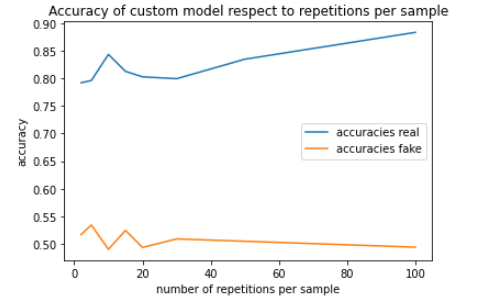
\includegraphics[width=\linewidth]{Accuracy-Repetitions.png}
        \caption{}
    \end{subfigure}
    \begin{subfigure}{0.49\textwidth}
	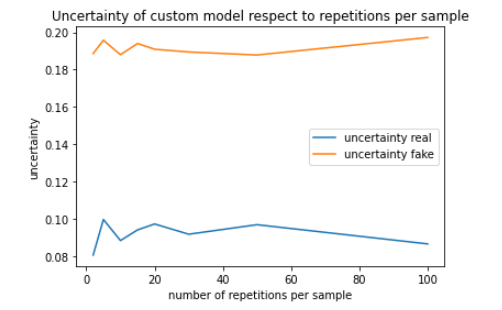
\includegraphics[width=\linewidth]{Uncertainties-Repetitions.png}
        \caption{}
    \end{subfigure}
    \caption{Accuracy and uncertainties of the UWL-BNN model as the number of predictions per step changes}
    \label{fig:n_predictions}
\end{figure}

The major drawback of the presented model is that it needs considerably more time to be trained. In fact, each forward pass is repeated multiple times, which leads to a linear increase in the training time. In order to provide some insights for future work, fig.~\ref{fig:n_predictions} shows how the performance of the model varies as the number of predictions is changed.

Tab.~\ref{tab:colab} provides an overview of the different models described in sec.~\ref{sec:models}. While the metrics are the same as in tab.~\ref{tab:custom}, it can be helpful to revise the differences between the models. The first one is a CNN trained on real samples only, with the purpose of providing a reference for how good the chosen network architecture solves the classification of histological images. The second model is a CNN trained both on real and spurious samples. The third model is a BNN, while the last model is the UWL-BNN introduced at the beginning of this section. Since the goal here is not to finetune a model, but to have a reliable metric of how good each model performs, the results in the table are computed using the test set.

Clearly, the CNN model trained on real samples performs best, since it does not have to deal with spurious images. Indeed, as soon as those are used at training time the accuracy drops drastically. When a BNN is used, the accuracy improves, probably because the class scores are computed as an average of multiple predictions. The BNN also produces an uncertainty measure through the use of Variational Dropout. At last, the UWL-BNN model achieves the best accuracy when spurious samples are present in the training set. Besides, it also has lower mean uncertainty for real samples as well as higher mean uncertainty for spurios ones.

\begin{table}[!t]
  \begin{adjustwidth}{-.5in}{-.5in}
  \begin{center}
    \begin{tabular}{l | c | c | c}
      Loss function	& Accuracy	& Uncertainty (real)	& Uncertainty (spurious) \\
      \hline
      CNN (real)	& 96,2 \%		& - 				& - \\      
      CNN		& 72,7 \%		& - 				& - \\      
      BNN		& 79,5 \%		& 10,4 \% 			& 19,9 \% \\      
      UWL-BNN		& 88,0 \%		& 9,1  \% 			& 20,0 \% \\       
    \end{tabular}
    \caption{Evaluation of different models}
    \label{tab:colab}
  \end{center}
  \end{adjustwidth}
\end{table}

\begin{figure}[!t]
    \centering
    \begin{subfigure}{0.30\textwidth}
	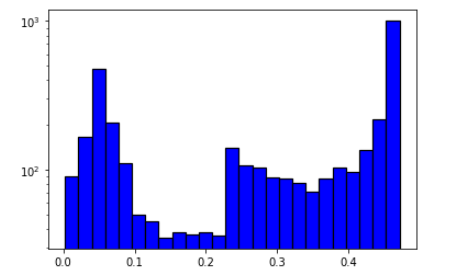
\includegraphics[width=\linewidth]{histo_CNN_all_real+fake.png}
        \caption{}
    \end{subfigure}
    \begin{subfigure}{0.30\textwidth}
	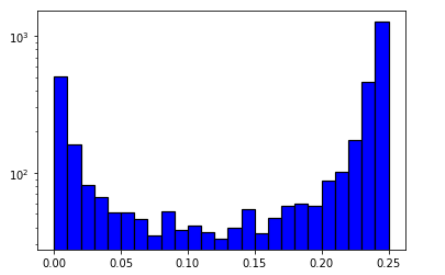
\includegraphics[width=\linewidth]{histo_BNN_all_real+fake.png}
        \caption{}
    \end{subfigure}
	\begin{subfigure}{0.30\textwidth}
	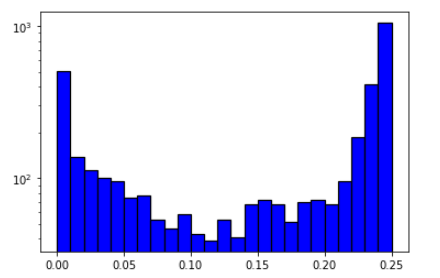
\includegraphics[width=\linewidth]{histo_Custom_all_real+fake.png}
        \caption{}
    \end{subfigure}
    \caption{Uncertainties computed by the CNN (a), BNN (b) and UWL-BNN (c) model on the whole dataset}
    \label{fig:histograms}
\end{figure}

\begin{figure}[!b]
    \centering
    \begin{subfigure}{0.49\textwidth}
	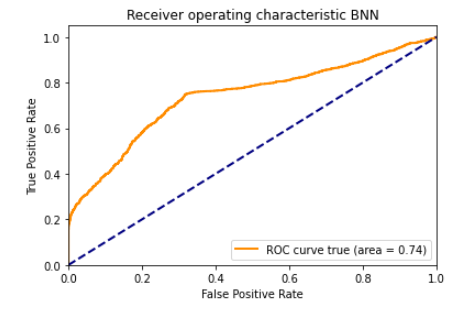
\includegraphics[width=\linewidth]{ROC_BNN.png}
        \caption{}
    \end{subfigure}
    \begin{subfigure}{0.49\textwidth}
	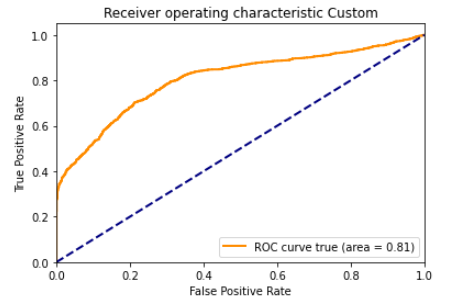
\includegraphics[width=\linewidth]{ROC_Custom.png}
        \caption{}
    \end{subfigure}
    \caption{Roc curves of the BNN (a) and UWL-BNN (b) model}
    \label{fig:roc}
\end{figure}

The uncertainty assigned by each model to the samples can be further analyzed by means of histograms, plotting how often the network outputs a value in a given range. Fig.~\ref{fig:histograms} shows such histogram for each of the three models trained on both real and spurious samples. In case of the CNN model the x-axis refers to the softmax uncertainty values obtained from the network output. It can be noticed that the BNN and the UWL-BNN models are capable of differentiating more between real and spurious samples, since they present higher peaks at the extreme values and lower plateaus in the middle. In fact, if a sample is assigned an uncertainty value in the middle range it is more difficult to predict for certain if it is real or not.

In case of the BNN, however, it is not straightforward to tell if it is capable of better differentiating real and spurious samples than the UWL-BNN or not (although a first clue is given by the mean uncertanties in tab.~\ref{tab:colab}). In other terms, it should be analyzed which of the two models allows to better recognize spurious samples using a single threshold with respect to the uncertainties.\newline
For this purpose, we consider a binary classification setting where the goal is to predict if a sample is real or spurious. In this setting, the uncertainty values can be considered as classification scores, i.e. they express the probability that a given sample is spurious. Now it is possible to compare the two models by considering their Roc curves with respect to this task. A Roc curve shows how true positives and false positives behave as the threshold in a binary classification changes. The greater the integral of the Roc curve (also called Area Under Curve, or Auc), the better the model.\newline
Fig.~\ref{fig:roc} shows the Roc curves of the BNN and the UWL-BNN model, respectively. It can be seen that the Auc of the UWL-BNN is 0.81, while the BNN only gets to 0.74. This confirms the hypothesis that the UWL-BNN is able of better differentiating real from spurious samples basing on their uncertainties.

\section{Conclusion}
The present work shows that the uncertainty measure computed in a BNN can be used in the training phase in order to improve the performance of the network at test time. However, this comes at a cost in term of resources: in particular, the time required to train the network increases proportionally to the number of predictions made at each step. While it is possible to overcome this issue in case of a small network such as the one presented in this work, it should be considered to which extent it is feasible to use this feature in bigger networks. Also, it could be interesting to further analyse the tradeoff between the number of predictions at each step and the performance of the network.\newline
A further line of future development would be to perform a separate finetuning for each model. In fact, in this work a single framework was used in order to provide a fair comparison between the models, however it could be possible to achieve a better performance by searching the best hyperparameters for each model. On the one hand, it is infeasible to fully scan the hyperparameter space, however a first step could be to explore different network architectures, learning rate schedules or number of epochs.

\bibliographystyle{plain}
\bibliography{bibliography} 

\end{document}

